\documentclass[10pt,twocolumn,letterpaper]{article}

\usepackage{cvpr}
\usepackage{times}
\usepackage{epsfig}
\usepackage{graphicx}
\usepackage{amsmath}
\usepackage{amssymb}
\usepackage{multirow}
\usepackage{algorithm}
\usepackage{algpseudocode}

\renewcommand{\algorithmicrequire}{\textbf{Input:}} % Use Input in the format of Algorithm
\renewcommand{\algorithmicensure}{\textbf{Output:}} % Use Output in the format of Algorithm

% Include other packages here, before hyperref.

% If you comment hyperref and then uncomment it, you should delete
% egpaper.aux before re-running latex.  (Or just hit 'q' on the first latex
% run, let it finish, and you should be clear).
\usepackage[breaklinks=true,bookmarks=false]{hyperref}

\cvprfinalcopy % *** Uncomment this line for the final submission

\def\cvprPaperID{****} % *** Enter the CVPR Paper ID here
\def\httilde{\mbox{\tt\raisebox{-.5ex}{\symbol{126}}}}

% Pages are numbered in submission mode, and unnumbered in camera-readyS
%\ifcvprfinal\pagestyle{empty}\fi
\setcounter{page}{1}
\begin{document}

%%%%%%%%% TITLE
\title{Discrimination of ADHD children based on Deep Bayesian Network}

\author{Junyu Hao\\
Department of Computer Technology\\
Tongji University\\
Shanghai, China\\
{\tt\small haojunyu2012@gmail.com}
% For a paper whose authors are all at the same institution,
% omit the following lines up until the closing ``}''.
% Additional authors and addresses can be added with ``\and'',
% just like the second author.
% To save space, use either the email address or home page, not both
\and
Lianghua He\\
Department of Computer Science and Technology\\
Tongji University\\
Shanghai, China\\
{\tt\small helianghua@tongji.edu.cn}
}

\maketitle
%\thispagestyle{empty}

%%%%%%%%% ABSTRACT
\begin{abstract}
Attention deficit hyperactivity disorder (ADHD) is a threat for the public health all the time, so the effective discrimination of it is significant and meaningful. In current research, Functional Magnetic Resonance Imaging (fMRI) data has become a popular tool for the analysis of ADHD. In this paper, we introduce the Deep Bayesian Network, a combination of Deep Belief Network and Bayesian Network, to classify the ADHD children from the normal. In Deep Bayesian Network, The Deep Belief Network is applied to  normalize and reduce dimension of the fMRI data in every brodmann area. And the Bayesian Network is used to extract the feature of relationships between several well-performed brain areas by structure learning. According to the information of structure and probability in Bayesian Network, we predicted the subjects as control,combined ,inattentive or hyperactive using SVM classifier. The final results perform better than using single Deep Belief Network and the best results in ADHD-200 competition. 
\end{abstract}



%%%%%%%%% BODY TEXT
\section{Introduction}

Attention deficit hyperactivity disorder (ADHD) is among the most common psychiatric disorders of childhood that persists into adulthood in the majority of cases\cite{1}. During this period, symptoms such as inattention, hyperactivity(restlessness in adults), disruptive behaviour, and impulsivity are common. Based on the presenting symptom, ADHD can be divided into three subtypes--predominantly inattentive, predominantly hyperactive impulsive or combined if criteria for both types are met. According to American Psychiatric Association’s Diagnostic and Statistical Manual, the prevalence of ADHD in the whole world is approximately 5\%, especially in the United States the prevalence among 8- to 15-years-olds reaches to 8.7\% during the past year. Therefore, the methods of diagnosing the ADHD is in urgent need.
 
 
 
Recently, Functional Magnetic Resonance Imaging(fMRI) has become very popular for brain activity related studies. Researchers use it for identifying the brain regions which are responsible for particular cognitive activities based on the correlation of input stimulus signal and captured brain fMRI signals. Shengfu Liang et al.\cite{3} utilizes the LDA classifier to discriminate children with ADHD by analyzing the resting-state functional magnetic resonance imaging (fMRI) data, and the average accuracy of distinguishing normal and ADHD children reaches 80.08\% though 50 times of 2-fold validation. Xunheng Wang\cite{4} applies Kernel Principal Component Analysis (KPCA) method based on connectivity matrix of each functional meaningful brain regions to find the abnormal pattern of ADHD. On this condition, Support Vector Machine (SVM) assifier make the correct classification rate reach about 81\% using a leave-one-out cross validation. On the global ADHD-200 competition, Eloyan A et al.\cite{6} from Johns Hopkins University mainly use rs-fc-fMRI based on decomposition of CUR along with gradient boosting. In the end, they achieved the best score. In this paper, three datasets from ADHD-200 competition are applied to discriminate ADHD with typical controls.

\begin{figure*}[ht]
\begin{center}
%\fbox{\rule{0pt}{2in} \rule{0.9\linewidth}{0pt}}
   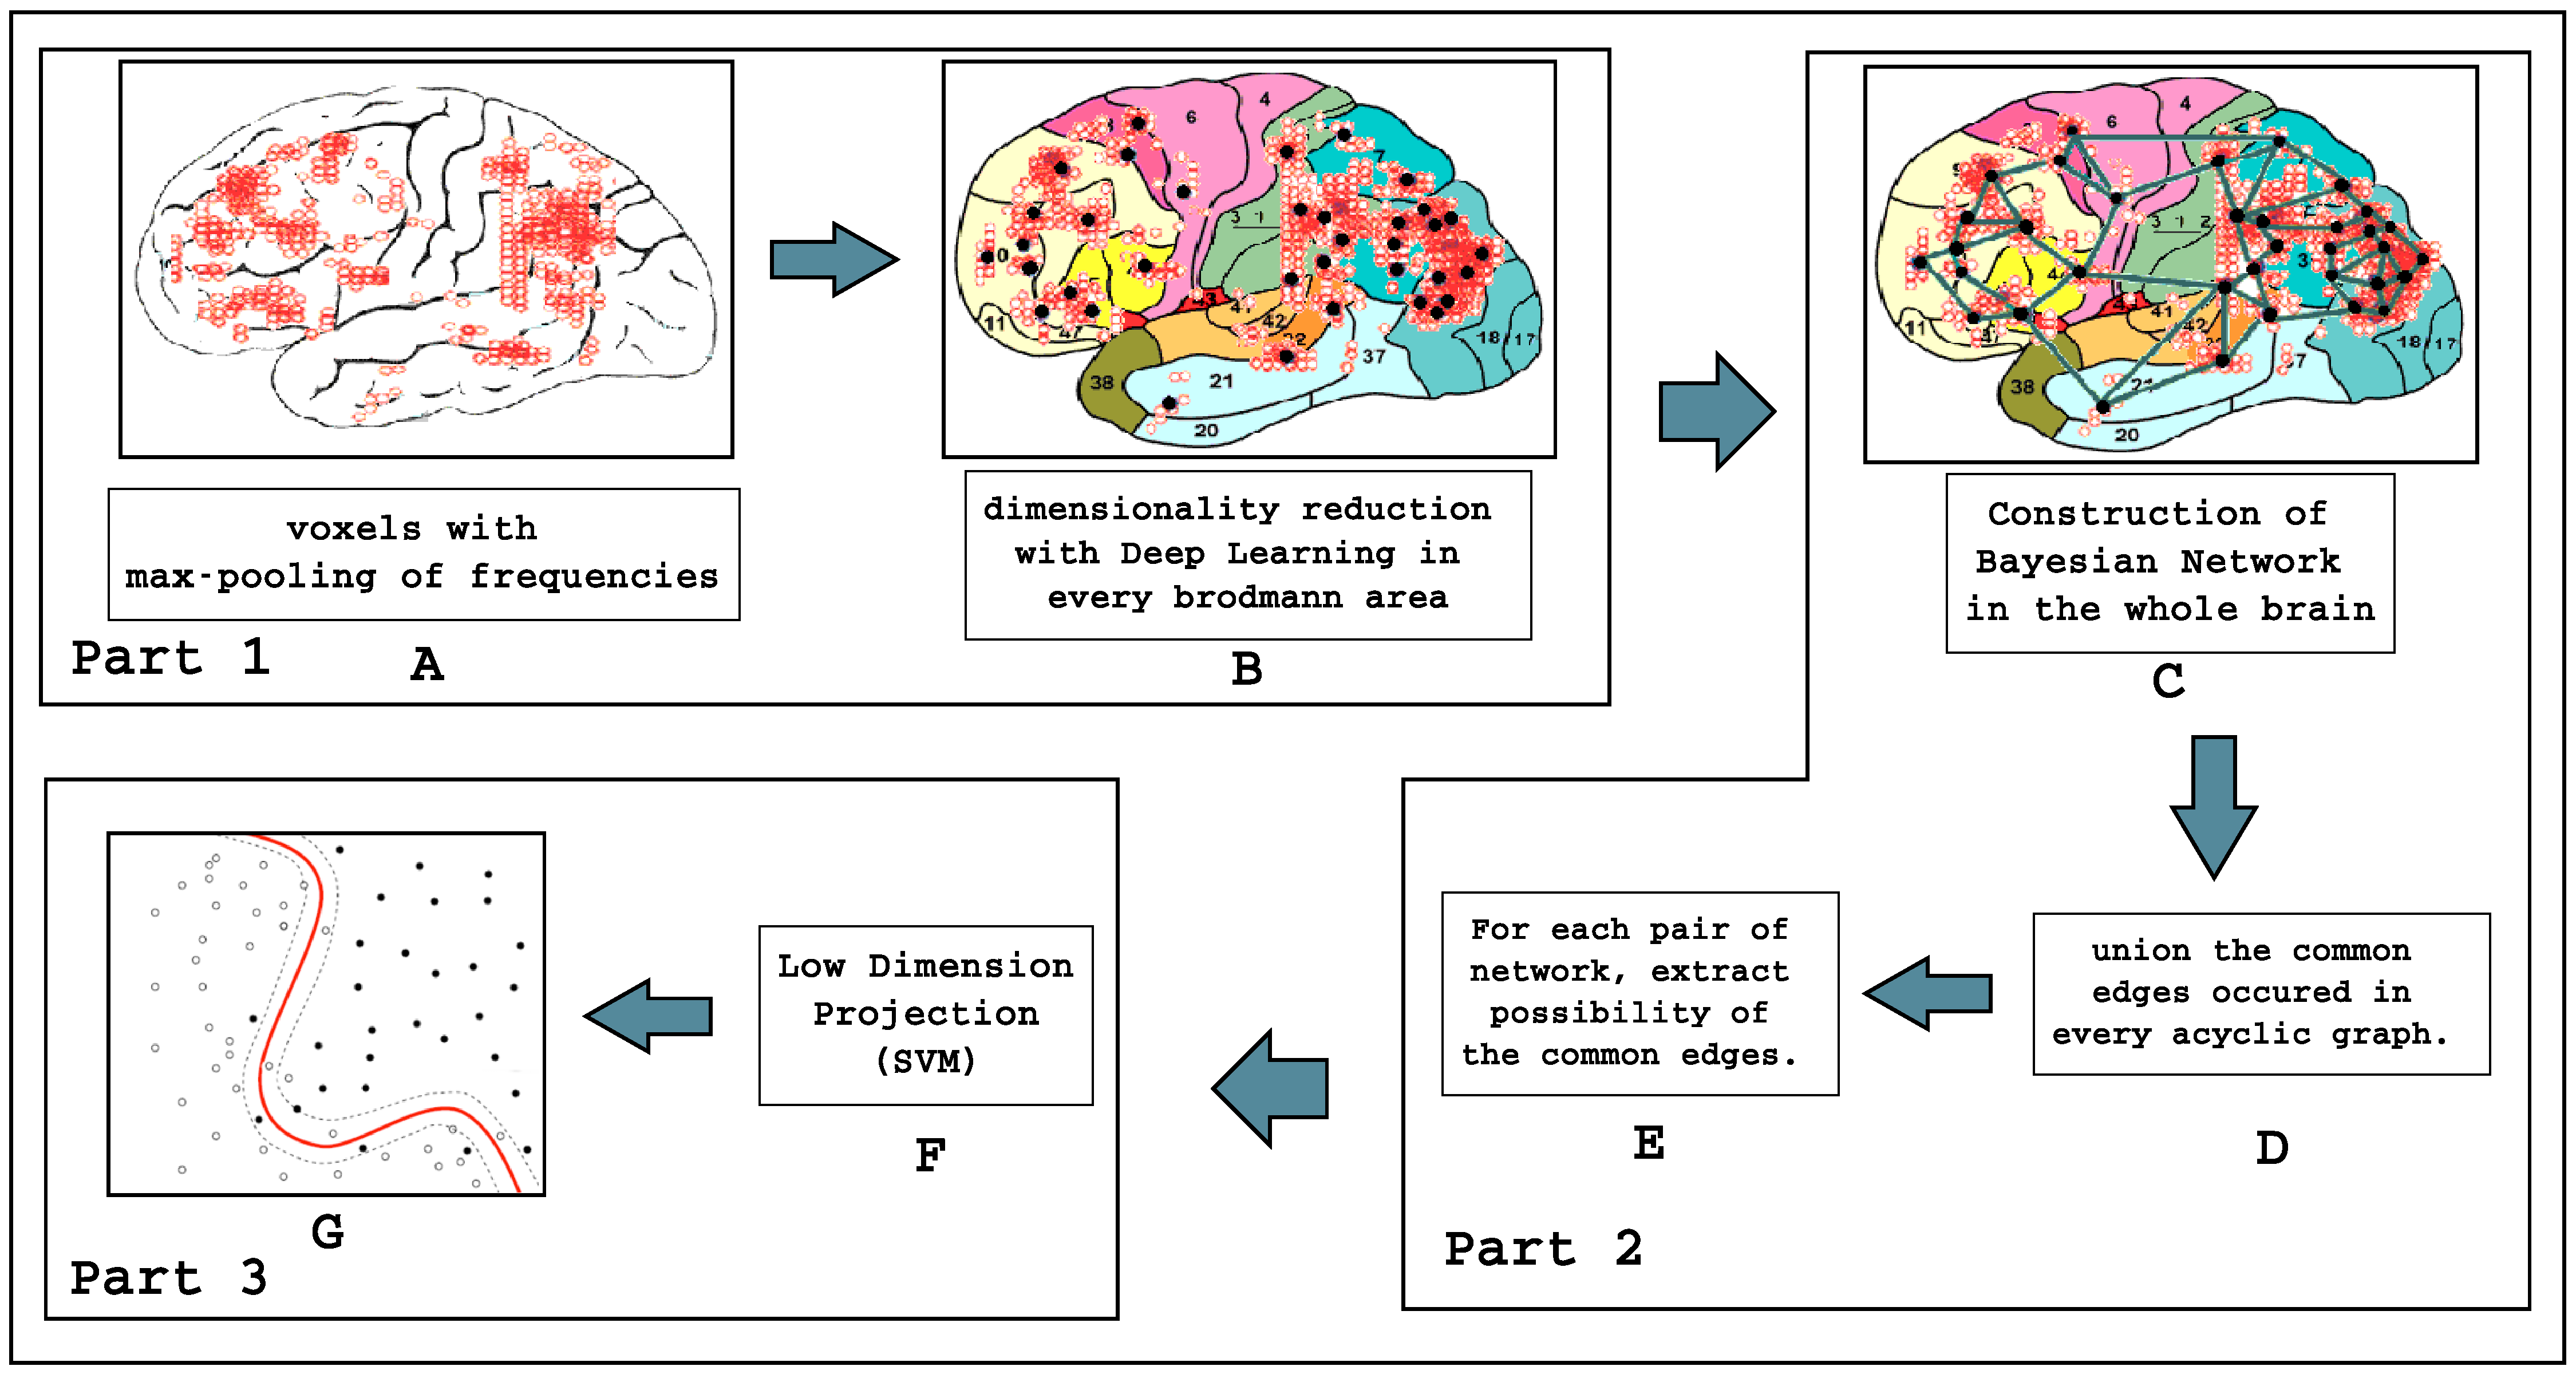
\includegraphics[width=0.8\linewidth]{overviews.eps}
\end{center}
   \caption{The procedure of Deep Bayesian Network}
\label{fig:overview}
\end{figure*}


As we all know, dimensionality reduction facilitates the classification and storage of high-dimensional data, especially for fMRI data in ADHD children. Compared with other method of reducing dimensionality, such as principal components analysis (PCA), Deep Belief Network not only perform better than them, but also can normalize the different number of voxels in different brodmann areas to the same size, which makes it possible that the data can be exactly dealt with Bayesian network. In addition, Geoffrey E.Hinton et al.\cite{8} derive a fast, greedy algorithm that can learn deep, directed belief networks one layer at a time, provided the top two layers form an undirected associative memory by using complementary prior.  In current, Deep Learning method has been applied for many areas including image processing \cite{8}, audio classification \cite{9}, natural language processing \cite{12} and so on. All of them achieved good performance. Considering its powerful learning ability and advantage of dimensionality reduction and normalization, Deep Learning method will be used to analysis massive fMRI data to dig out the cognitive significance of brain in this paper.


To reduce the complexity of computation, the fMRI data, which is a time series of 3D images, is divided into 48 areas according to brodmann template. Due to the cause in ADHD cases is unknown, we should take all the brain areas into consideration rather than analysis the brain area separately, which meets the requirement of Bayesian network. Besides, it is a graphical model that can encodes probabilistic relationships among variables of interest. On one hand, the model can be used to learn causal relationships, and hence can be used to gain understanding about a problem domain and to predict the consequences of intervention. For example, in bioinformatics learning Bayesian networks have been used for the interpretation and discovery of gene regulatory pathways \cite{14}. On the other hand, it has both a causal and probabilistic semantics, it is an ideal representation for combining prior knowledge (which often comes in causal form) and data. Based on this, Bayesian network has been used in information retrieval\cite{15}, natural language processing\cite{16}, and for the analysis of a medical service’s performance for management decisions\cite{17}. In this paper, Bayesian network is applied to retrieval the information between different brain areas, which is shown by the edges in the graph of the Bayesian network.  

 

This paper will introduce the Deep Belief Network as a tool to reduce the dimensionality of data. Before this, the frequency feature on the voxels of the different brain areas(\textbf{A} in Fig.\ref{fig:overview}) are used as a vector of feature for the raw input for the Deep Belief Network. Besides, Deep Belief Network can reconstruct the different number of voxels in different areas into the same number of features(\textbf{B} in Fig.\ref{fig:overview}). This normalization of fMRI data make it possible that Bayesian network can extract the relationships from different brain areas(\textbf{C-E} in Fig.\ref{fig:overview}). Finally, using SVM as a classifier to discriminate the ADHD children from normal(\textbf{F-G} in Fig.\ref{fig:overview}). The flow chart of the whole procedure is shown in Figure \ref{fig:overview}.

Results show that the method proposed in this paper got better performance than the competition and the Deep Belief Network single. Section 2 mainly describes the Deep Belief Network method, Bayesian network and the application of two graph model for ADHD data. Section 3 presents our experiments and results on ADHD dataset.



\section{METHOD}
The proposed method, Deep Bayesian Network, can be divided into three main parts such as Deep Belief Network for  normalization and Dimensionality reduction(Part 1 in Fig.\ref{fig:overview}), Bayesian Network construction for feature extraction(Part 2 in Fig.\ref{fig:overview}), SVM for ADHD subject classification(Part 3 in Fig.\ref{fig:overview}). The following sections describe each of the parts in details.


\subsection{Deep Belief Network}
Deep Belief Network is composed of a stack of
restricted Boltzmann machines (RBM) which is shown in Figure~\ref{fig:DBN}.
\begin{figure}[ht]
\begin{center}
%\fbox{\rule{0pt}{2in} \rule{0.9\linewidth}{0pt}}
   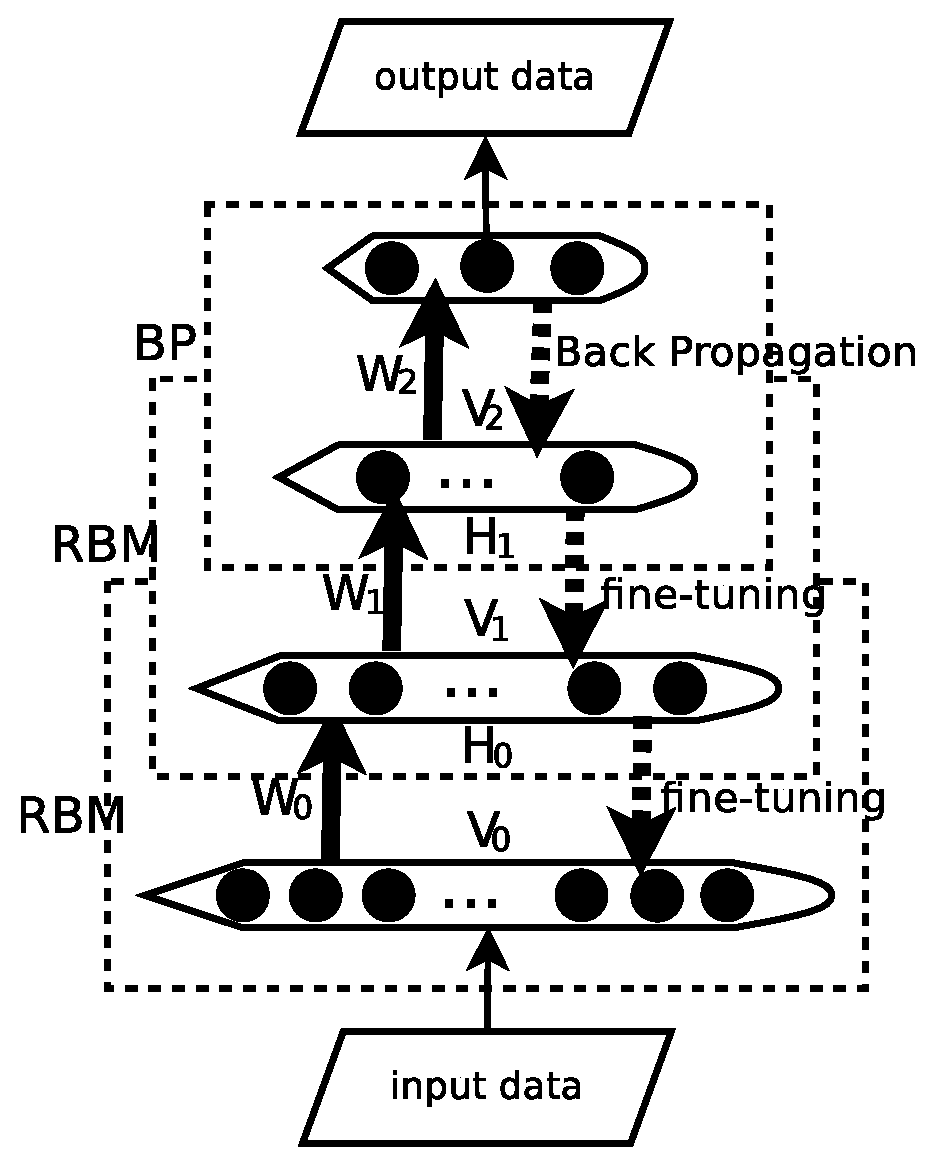
\includegraphics[width=0.755\linewidth]{DBN.eps}
\end{center}
   \caption{Architecture of Deep Belief Network}
\label{fig:DBN}
\end{figure}
Training the architecture of Deep Belief Network includes two steps, which are pretraining and back propagation. Pretraining each layer of RBM network make sure that the feature can be mapped into different feature space and keep more feature information at the same time. Back propagation spread the error message to every level of RBM from the top to down. This procedure is viewed as a initialization of parameter weights, which overcome the shortcomings of local optimum and long train time due to random initializtion of parameter weights. 



As a component of Deep Belief Network, the restricted Boltzmann machine \cite{13} is a two-layer, undirected, bipartite graphical model where the first layer consists of observed data variables (or visible units), and the second layer consists of latent variables (or hidden units). The visible and hidden layers are fully connected via symmetric undirected weights, and there are no intra-layer connections within either the visible or the hidden layer. A typical RBM model topology is shown in Figure ~\ref{fig:RBN}.
\begin{figure}[ht]
\begin{center}
%\fbox{\rule{0pt}{2in} \rule{0.9\linewidth}{0pt}}
   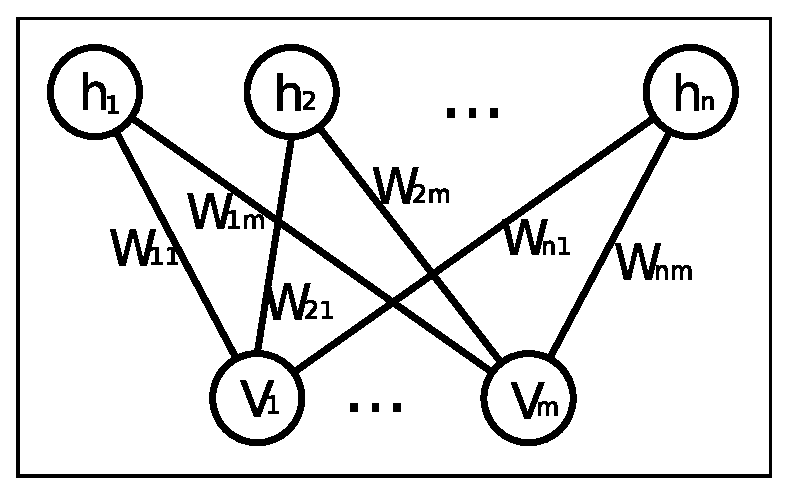
\includegraphics[width=0.8\linewidth]{RBN.eps}
\end{center}
   \caption{Struct of RBM}
\label{fig:RBN}
\end{figure}

The weights and biases of an RBM determine the energy of
a joint configuration of the hidden and visible units $E(v,h)$,
\begin{equation}
E(v,h;\theta) = -\sum_{i=1}^V \sum_{j=1}^H v_ih_jw_{ij} - \sum_{i=1}^V b_iv_i - \sum_{j=1}^H a_jh_j
\end{equation}
with model parameters $\theta = \{W,b,a\}$ and $v_i,h_j \in \{0,1\}$. $W$ are the symmetric weight parameters with $V * H$ dimensions, $b$ are the visible unit bias parameters, $a$ are the hidden unit bias parameters.

In general Boltzmann machines, the probability distributions
over hidden and visible units are defined in terms of the energy function:
\begin{equation}
p(v,h) = \frac{1}{z} \exp ( -E(v,h) )
\end{equation}
where $z$ is defined as the sum of $\exp ( -E(v,h) )$. Based on the joint probability of $v$ and $h$, the conditional probability of $v$ given $h$ and of $h$ given $v$ is easily obtained. So the individual activation probabilities are given by
\begin{equation}
p(h_j = 1 | v) = \alpha(\sum_{i=1}^m w_{ij}v_i + a_j) 
\end{equation}
\begin{equation}
p(v_i = 1 | h) = \alpha(\sum_{j=1}^n w_{ij}h_j + b_i) 
\end{equation}
where $\alpha(t) = (1 + \exp(-t))^{-1}$.

A RBM is pre-trained to maximize the log-likelihood $\log P(v)$.Following the gradient of the log likelihood we obtain the update rule for the weights as,
\begin{equation}
\Delta w_{ij} = \epsilon (<v_i,h_j>_{data} - <v_i,h_j>_{recon})
\end{equation}
Where $\epsilon$ is the learning rate and the angle brackets manifests the expectations relative to the distribution specified in the subscript. The updating rule makes it the reconstruction of hidden units equals to the data. Only by this way, the hidden unit is approximate to the visible units. Then they can be seen as the exact expression of the data.



\subsection{Bayesian Network}
Bayesian Network includes a directed acyclic graph (DAG) and a condition probability table related to every node (CPT). The fronter is called network structure learning, and the other is called parameters learning. This paper mainly uses the structure to extract the information, so we will pay more attention on structure learning, which can find the best Bayesian network which is most suitable to the brain areas.
The directed acyclic graph (DAG) can expresses the factorization property of a joint distribution p(x). With each variable corresponding to a node in $\mathcal{G}$, the joint distribution is factorized as 
\begin{equation}
p(x) =\prod_{i=1}^m p(x_i |\boldsymbol{Pa}(x_i))
\end{equation}
where $\boldsymbol{Pa}(x_i)$ denotes the parent $i=1,\cdots,m$ nodes of $x_i$ .


Currently, there are three methods to learn the structure of Bayesian network, which are method based on searching and scoring, method based on testing independence and the mix of two. The third method performs well, especially for Max-Min Hill Climbing(MMHC) algorithm. MMHC algorithm can be divided into two stages. Firstly, probable parent nodes of each node  have to be determined, which can determine the initial Bayesian network architecture. Secondly, use search-and-score method to determine the relationship between each node. For the variable $x$, Max-Min Parents and Children (MMPC) algorithm will determine the candidate set of parent nodes in the first stage, which is call $CPC(x)$, If another variable $a$ meet this condition $a \in CPC(x)$, what we can determine is that there is a undirected edge between x and a, but the direction is uncertain. In this way, MMPC algorithm can determine the preliminary framework of undirected network. In order to determine the exact relationship between each node, search-and-score method performs the operations of adding, subtracting and reversing the edge to change the structure of the network, and scores each network to find the best one. The difference between MMHC and Greedy searching algorithm is that searching space is just limited to the case when variable $a$ belongs to $CPC(x)$, MMHC algorithm will add an edge from $a$ to $x$. By this, MMHC can reduce the searching spaces and  improve the learning efficiency of the whole algorithm. In the end, we can get a DAG and the condition probability of each edge, which is shown in Figure 
\begin{figure}[ht]
\begin{center}
%\fbox{\rule{0pt}{2in} \rule{0.9\linewidth}{0pt}}
   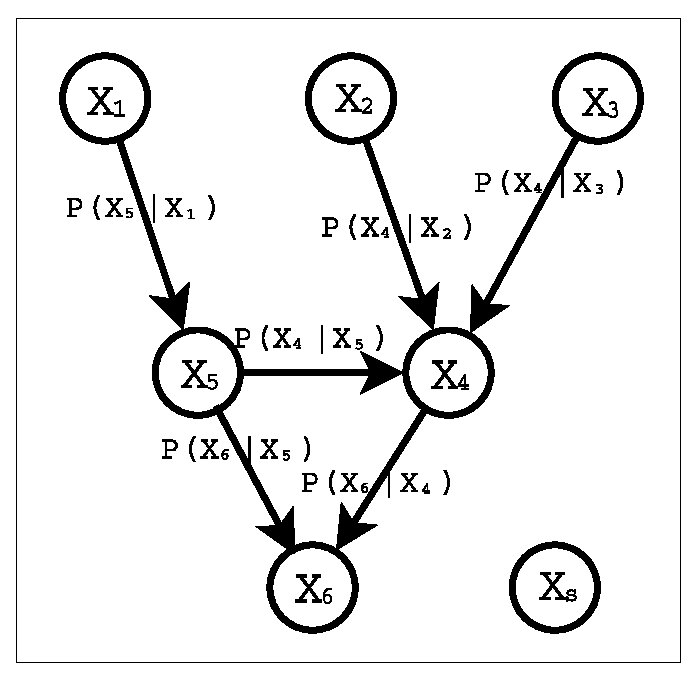
\includegraphics[width=0.68\linewidth]{DAG.eps}
\end{center}
   \caption{Struct of Bayesian Network}
\label{fig:BN}
\end{figure}


%-------------------------------------------------------------------------
\subsection{The Construction of Deep Bayesian Network}
Deep Bayesian Network includes two parts. One is Deep Belief Network which is applied to normalize and reduce the dimensionality of fRMI data in different Brodmann areas of ADHD. The other one is Bayesian network,which is used to train everyone's data to find the information of relationships between the different brodmann areas in order to distinguish the ADHD person from normal.

\subsubsection{Deep Feature Extraction}
To extract and normalize the deep feature, Deep Belief Network  is applied to this. But before DBN, some preprocessing are needed for the fMRI data, such as realign, slice time, co-register, normalize, smooth which are described in this paper\cite{18} in detail. First, according to brodmann template, the 3D images of fMRI datas $X$ are divided into 48 areas, where divided data $X_d$ is a 1*48 cell array. In every cell, $X_d$ have the same data structure as the orginal data $X$. Second, transform the divided data $X_d$ from time domain to frequency domain by the fast Fourier transform algorithm (FFT). 
\begin{equation}
X_{fft} = fft(X_d)
\end{equation}
third, execute max-pooling of frequencies in each voxel to select the frequency which has the maximum value of voxels in some areas may be different during the scanning procedure and the frequency is higher when the voxel is more active. At this time, each voxel has only one property and the number of properties in each brain areas depends on the number of voxels, which is present as $X_{max}$. That is to say, after preprocessing, the DBN architecture with three hidden layers convert the datas from $X_{max} (48*n)$  to $X_{dbn} (48*50)$, where n is changeable and represents the number of voxels in different brain areas. The pseudo-code for application of Deep Belief Network on ADHD data can be seen as following Algorithm \ref{code:DBN} .
\begin{algorithm}[h]
\caption{Deep Feature Extraction}
\label{code:DBN}
\begin{algorithmic}[1]
\Require
$X$

\State $initial()$;\Comment{$maxepoch,vhn,tn$}
\State $X_{max} \gets preprocess(X)$ \Comment{preprocess data} 
\For{$k \gets 1, 3$} \Comment{train the weights of rbm}
\State $[\theta,X_{tmp}]\gets RBN(X_{max})$ \Comment{train $\theta=[w,vb,hb]$}
\State $X_{max} \gets X_{tmp}$ \Comment{update data}
\EndFor
\State $backprop(\theta,X_{max})$ \Comment{back propagation}
\State $X_{dbn} \gets DBN(\theta,X_{max})$ \Comment{reduce dimensionality}
\Ensure
$X_{dbn}$
\end{algorithmic}
\end{algorithm}



\subsubsection{Structure Learning of Deep Bayesian Network}
To extract the feature of relationships between different brain areas, the structure learning of Deep Bayesian network is applied to solve this. But before constructing Deep Bayesian Network, some preprocessing are needed for the data from Deep Bayesian Network.


First, the input data $X_{dbn}$ need to be filtered so that it can be wipe out the noise. Second, the MMHC algorithm can speed up the structure of Bayesian network, but it needs the limited parent nodes of each node. So the dependent nodes $K$ are treated as the limited parent nodes computing by conditional independence testing in filtered data $X_{filter}$. Third, we union the limited parent nodes and use it $K_{un}$ to learn the structure of all data including training data and testing data. By this, we can get a DAG $G$ and a table $P$ including the information of probability of edge between the two nodes. Forth, the probabilities of each edge in Bayesian network will be exacted out and viewed as feature $F$ of ADHD children and normal children. Finally, SVM will be acted as classifier to train the training sample, which will get the structure parameter of the mode $S_{mod}$, and classify the testing sample, which will get the predicted label of testing sample $L$. The accuracy $T$ can be computed by predicted labels $L$ and true labels $Y$. The pseudo-code for application of BN on ADHD data can be seen as following Algorithm \ref{code:BN}.  
\begin{algorithm}[h]
\caption{Structure Learning of Deep Bayesian Network}
\label{code:BN}
\begin{algorithmic}[1]
\Require
$X_{dbn},Y$

\State $X_{filter} \gets preprocess(X_{dbn})$ 

\State $K \gets indep(X_{filter})$ \Comment{Conditional independence test}
\State $K_{un} \gets union(K)$ \Comment{union the parent's limitation}
\State $ [G,P] \gets BN(K_{un},X_{filter})$ \Comment{structure learning}
\State $F \gets extract(G,P)$ \Comment{extract feature}
\State $S_{mod} \gets svmtrain(F,Y)$ \Comment{svm training}
\State $L \gets svmpre(S_{mod},P)$ \Comment{svm predicting}
\State $T \gets com(Y,L)$ \Comment{compute the accuracy}

\Ensure
T
\end{algorithmic}
\end{algorithm}





\section{EXPERIMENTS AND RESULTS}
\subsection{Data}
The data used in this paper can be downloaded from the ADHD-200 Global Competition website. DBN and BN model is built upon the ADHD dataset for NYU, Peking-1 and KKI respectively.


For NYU, the training subjects are 216, and testing subjects are 41; for Peking-1 dataset, the training subjects are 85, and testing subjects are 50; and for KKI the training subjects and testing subjects are 83 and 11 respectively. The detail information for the subjecets is shown in Table ~\ref{tab:Information}.


\begin{table}[h]
\label{tab:Information}
\begin{center}
\begin{tabular}{|c|c|c|c|c|c|c|}
\hline
\multirow{3}{*}{site}	& \multicolumn{2}{c|}{NYU} & \multicolumn{2}{c|}{Peking-1} & \multicolumn{2}{c|}{KKI} \\
\cline{2-7}\rule{0pt}{5pt}
					 	& train &  test  & train	& test 	& train & test  \\
						& 216	& 41	  &    85   &   50  &   83   &   11 \\ [2pt]
\hline \rule{0pt}{12pt}
control					& 98	    & 7    &    61   &    27 &   61    &   8 \\
combined					& 73		& 22   &    7    &    9  &   16    &   3 \\
inattentive				& 2		& 0    &    0    &    1  &   5     &   0 \\
hyperactive				& 43		& 7    &    17   &    13 &   1    &   0 \\[2pt]
\hline
\end{tabular}
\end{center}
\caption{Demographic Information of three Datasets}
\end{table}



\subsection{The Experiment of Parameter Designing}
To construct a Deep Bayesian Network, we must set up the number of selected brain areas. If the parameter of number is small, the Bayesian network will can't extract the enough information of relationships between brain areas from the structure. If the parameter of number is too large, the probability of that unrelated brain areas will be chose as a node will get higher, which has a side effect on the final classification. In addition,  with the increase of the variables, the search space of network structure will presents exponentially. So the experiment of parameter designing is significant.
\subsubsection{Accuracy in Single Brain Area}
As NYU dataset in the ADHD-200 competition achieved the lowest discrimination results, Deep Belief Network algorithm is particularly tested on the NYU dataset of 48 areas and softmax as a classifier generates the accuracies of different brain areas,which is convenient for the choice of node in the Bayesian network. The results of 48 regions are shown in Figure~\ref{fig:NYU}.
\begin{figure}[ht]
\begin{center}
%\fbox{\rule{0pt}{2in} \rule{0.9\linewidth}{0pt}}
   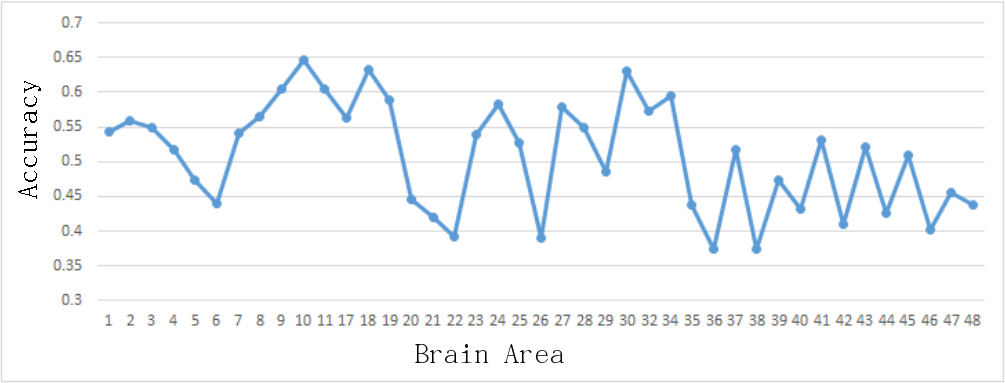
\includegraphics[width=0.9\linewidth]{NYU.png}
\end{center}
   \caption{Accuracy of NYU in 48 Areas}
\label{fig:NYU}
\end{figure}


From the figure above, we can see that different brain areas have different performance of discriminate the ADHD children from the normal. The area of 9, 10 , 11, 18, 30 perform well. According to brodmann definition, area 9, 10, 11 stands for prefrontal cortex, area 18 plays a role in the visual cortex and area 30 is part of cingulate cortex.


\subsubsection{Accuracy of Several Brain Area}
As we all know, Bayesian network can extract the feature of relationships between brain areas. Obviously, selecting the well-performed brain areas first in current is a good strategy. According to Figure ~\ref{fig:NYU}, the performance in ares of 10, 18, 30, 9, 11, 19, 34, 32, 8, 17, 2, 28, 3, 1, 7, 23, 25, 41 decreases step by step. The result of different number of areas by BN is shown in Figure ~\ref{fig:BN}. 
\begin{figure}[ht]
\begin{center}
%\fbox{\rule{0pt}{2in} \rule{0.9\linewidth}{0pt}}
   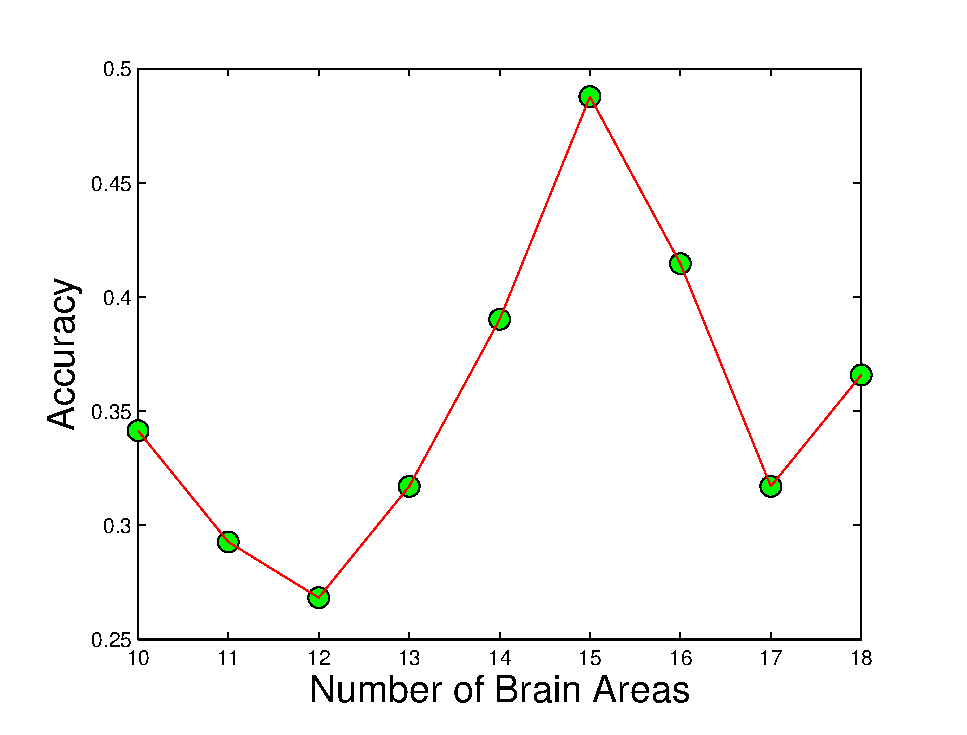
\includegraphics[width=0.7\linewidth]{BN.eps}
\end{center}
   \caption{Accuracy in Different Number of Brain Areas}
\label{fig:BN}
\end{figure}


From the chart we can see that the accuracy of discriminate fluctuate a little from 10 to 18, but it reaches the peak when the number of brain areas is equal 15. So we will choose 15 brain areas in the front to construct the Bayesian network. Besides, using the relationships between brain areas to discriminate ADHD is better than using information in single brain area and the best result in  ADHD-200 competition.


\subsection{Performances on NYU, Peking-1 and KKI dataset}
The experiments are also excuted on the NYU, Peking-1 and KKI dataset. The results released by ADHD-200 competition are 35.19\% for NYU, 51.05\% for Peking-1 and 61.90\% for KKI respectively. The prediction accuracies of Attributed graph distance\cite{19} (AGD) are none, 58.82\%,54.55\%. The Deep Bayesian Network  gain a higher prediction accuracies than Deep Belief Network single, which are 48.78\% for NYU, 54.00\% for Peking-1 and 72.72\% for KKI. The details show in Figure ~\ref{fig:dataset}.
\begin{figure}[ht]
\begin{center}
%\fbox{\rule{0pt}{2in} \rule{0.9\linewidth}{0pt}}
   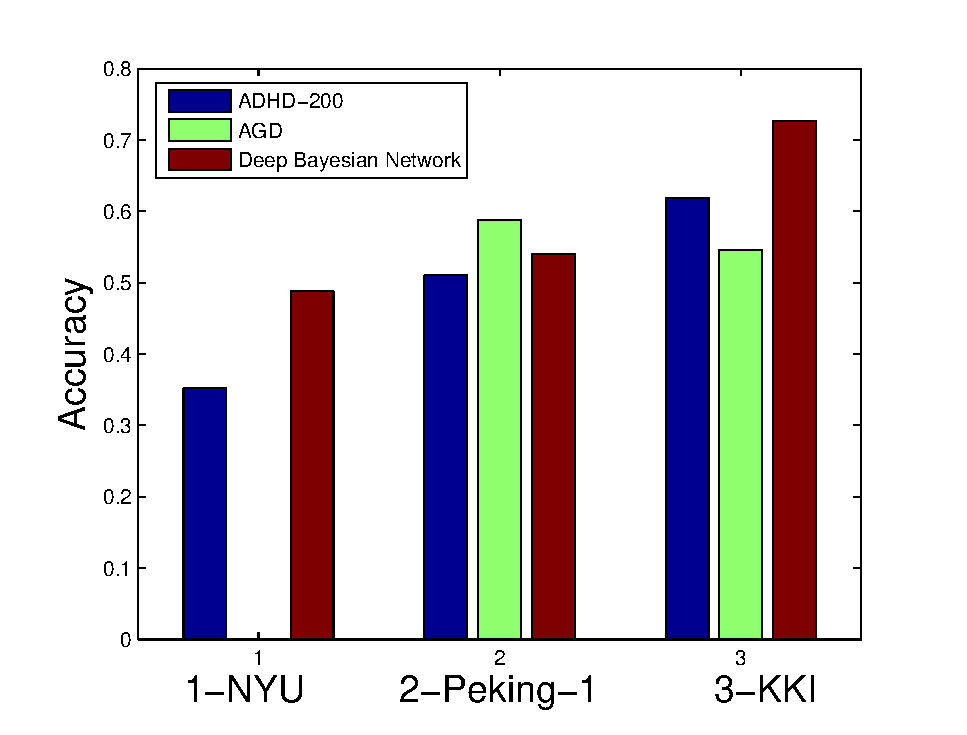
\includegraphics[width=0.7\linewidth]{Datasets.eps}
\end{center}
   \caption{Performance in Different Datasets}
\label{fig:dataset}
\end{figure}


From this chart, we can see that Deep Bayesian Network improves the prediction accuracies  in these three datasets  compared with the results of ADHD-200 competition. Besides, the increase of accuracy is the highest in the NYU dataset than other two dataset. Table ~\ref{tab:Information} shows us that the number of training samples in NYU dataset is far more than Peking-1 and KKI. So Bayesian network can extract more useful feature of relationships between brain areas. The different number of training samples can have a big effects on the accuracy. This effect is shown in Figure ~\ref{fig:Number}.
\begin{figure}[ht]
\begin{center}
%\fbox{\rule{0pt}{2in} \rule{0.9\linewidth}{0pt}}
   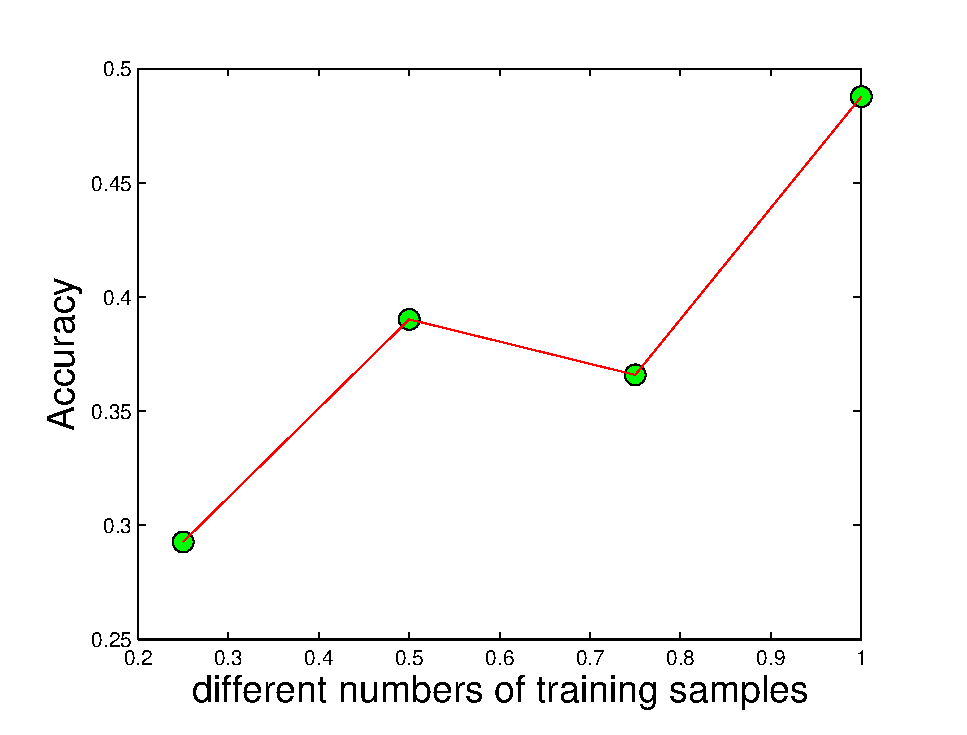
\includegraphics[width=0.7\linewidth]{Number.eps}
\end{center}
   \caption{Performance in Different Number of training samples}
\label{fig:Number}
\end{figure}



Considering that discriminating the ADHD is important and meaningful, here we take the prediction accuracy of the method along with the specificity and sensitivity values into consideration. The detail information is show in Tab \ref{tab:2}.

%NYU			&  -		&   -	 &  - &  64.65	&  68.77 & 43.89 \\[2pt]
%Peking-1		& 58.82		&  92.59 	& 20.83 & 66.32 & 87.71 &22.88\\[2pt]
%KKI			& 54.55		& 62.50	& 33.33 & 58.96  & 82.98  & 55.56\\[2pt]


\begin{table}[h]
\label{tab:2}
\begin{center}
\begin{tabular}{cccc}
\hline

Dataset  	&   Accuracy  	&	Specificity  &	Sensitivity \\
\hline
NYU			&  64.7	&  68.8 & 43.9 \\[2pt]
Peking-1		& 66.3 & 87.7 &22.9\\[2pt]
KKI			& 59.0  & 83.0  & 55.6\\[2pt]
\hline
\end{tabular}
\end{center}
\caption{The Detail information in Different Datasets}
\end{table}







%------------------------------------------------------------------------
\section{CONCLUSION}
In this paper, Deep Bayesian Network, which is a mix of Deep  Belief Network and Bayesian Network, is introduced to discriminate the ADHD children from the normal. Deep Belief Network as a one of the Deep Learning models can be better applied for reducing dimensionality and normalizing the fMRI data. In addition, Bayesian Network is used to extract the feature of relationships between the selected brain areas. During the procedure, the number of perform-well brain areas is discussed in order to find the best value of this parameter.


In the future, we could find more effective method to choose the different brain areas as the input of Bayesian Network. In addition, the distance between different brain areas is different, so they have different influence over each other. we could take  the area's neighborhood into consideration manually to strengthen the structure learning.



%-------------------------------------------------------------------------
\section{ACKNOWLEDGMENT}

This work was supported by National Natural Sciences
Foundation of China (No.61272267, 61270220, 51075306,
61273261), Program for New Century Excellent Talents in
University (NCET-11-0381), Fundamental Research Funds for
the Central Universities, State Key Laboratory of Software
Engineering.




%-------------------------------------------------------------------------



{\small
\bibliographystyle{ieeetr}
\bibliography{egbib}
}

\end{document}
